\documentclass[]{article}
\usepackage{lmodern}
\usepackage{amssymb,amsmath}
\usepackage{authblk}
\usepackage{blindtext}
\usepackage{graphicx} 
\usepackage{subfigure} 
\usepackage{ifxetex,ifluatex}
\usepackage{fixltx2e}
\usepackage[hidelinks]{hyperref}
\ifnum 0\ifxetex 1\fi\ifluatex 1\fi=0 % if pdftex
  \usepackage[T1]{fontenc}
  \usepackage[utf8]{inputenc}
  \usepackage{authblk}

\else % if luatex or xelatex
  \ifxetex
    \usepackage{mathspec}
  \else
    \usepackage{fontspec}
  \fi
  \defaultfontfeatures{Ligatures=TeX,Scale=MatchLowercase}
\fi
% use upquote if available, for straight quotes in verbatim environments
\IfFileExists{upquote.sty}{\usepackage{upquote}}{}
% use microtype if available
\IfFileExists{microtype.sty}{%
\usepackage{microtype}
\UseMicrotypeSet[protrusion]{basicmath} % disable protrusion for tt fonts
}{}
\usepackage[margin=1in]{geometry}
\usepackage{hyperref}
\hypersetup{unicode=true,
            pdftitle={Informe Presentación Profesor},
            pdfauthor={Francisco Javier Flores Gajardo} ,
            pdfborder={0 0 0},
            breaklinks=true}
\urlstyle{same}  % don't use monospace font for urls
\usepackage{graphicx,grffile}
\makeatletter
\def\maxwidth{\ifdim\Gin@nat@width>\linewidth\linewidth\else\Gin@nat@width\fi}
\def\maxheight{\ifdim\Gin@nat@height>\textheight\textheight\else\Gin@nat@height\fi}
\makeatother
% Scale images if necessary, so that they will not overflow the page
% margins by default, and it is still possible to overwrite the defaults
% using explicit options in \includegraphics[width, height, ...]{}
\setkeys{Gin}{width=\maxwidth,height=\maxheight,keepaspectratio}
\IfFileExists{parskip.sty}{%
\usepackage{parskip}
}{% else
\setlength{\parindent}{0pt}
\setlength{\parskip}{6pt plus 2pt minus 1pt}
}
\setlength{\emergencystretch}{3em}  % prevent overfull lines
\providecommand{\tightlist}{%
  \setlength{\itemsep}{0pt}\setlength{\parskip}{0pt}}
\setcounter{secnumdepth}{0}
% Redefines (sub)paragraphs to behave more like sections
\ifx\paragraph\undefined\else
\let\oldparagraph\paragraph
\renewcommand{\paragraph}[1]{\oldparagraph{#1}\mbox{}}
\fi
\ifx\subparagraph\undefined\else
\let\oldsubparagraph\subparagraph
\renewcommand{\subparagraph}[1]{\oldsubparagraph{#1}\mbox{}}
\fi

%%% Use protect on footnotes to avoid problems with footnotes in titles
\let\rmarkdownfootnote\footnote%
\def\footnote{\protect\rmarkdownfootnote}

%%% Change title format to be more compact
\usepackage{titling}

% Create subtitle command for use in maketitle
\providecommand{\subtitle}[1]{
  \posttitle{
    \begin{center}\large#1\end{center}
    }
}

\setlength{\droptitle}{-2em}
%Informe Presentación Profesor Feijoo Tema: 
  \title{Informe Presentación Profesor Orlando Duran}
    \pretitle{\vspace{\droptitle}\centering\huge}
  \posttitle{\par}
  \author{Belén Vergara Yantén}
    \affil[1]{Industrial PhD Program; School of Industrial Engineering; Pontificia Universidad Católica
de Valparaíso.}
    \preauthor{\centering\large\emph}
  \postauthor{\par}
    \date{}
    \predate{}\postdate{}
  
  
\usepackage{pgf,tikz}

\begin{document}
\maketitle




\hypertarget{introducccion-descripcion-general}{
\section{Introduccción }
\label{introducccion-descripcion-general}}

El profesor Ph.D. Ing. Orlando Duran, actualmente docente de las Carreras Ingeniería Civil mecánica e Ingeniería mecánica de la Pontificia universidad católica de Valparaíso, también parte del cuerpo Docente del Programa de Doctorado de Ingeniería industrial, además de realizar módulos en diversos magister y diplomados a nivel nacional, tiene como áreas de especialización:

\begin{itemize}
    \item 	Automatización de la Manufactura 
    \item	Procesos con arranque de viruta
    \item   Ingeniería artificial
    \item	Optimización de procesos 
\end{itemize}

Las Publicaciones del Profesor Duran son cerca de 80, en los cuales ha obtenido mas de 600 citaciones y un poco más de 8.000 lectores de estas investigaciones. De las publicaciones antes mencionadas, podríamos destacar las siguientes:

\begin{enumerate}
    \item 	A TD-ABC Model for the Computation of the Total Cost of Ownership of Spare Parts
Marzo de 2020 Paper de Paulo Alonso y el Profesor Orlando Duran.



“Los costos de las piezas de repuesto representan una parte importante de los costos de operación y mantenimiento de los bienes de capital. Las piezas de repuesto pueden permanecer en depósitos y almacenes durante largos períodos de tiempo, y muchas de ellas requieren actividades logísticas. Existen varios modelos de estimación de costos de ciclo de vida para sistemas de producción intensivos en capital, sin embargo, comúnmente, no consideran los costos de logística adecuadamente. Por lo tanto, para incorporar todos estos aspectos en el cálculo del costo de propiedad de las piezas de repuesto, en este documento se propone un modelo de costos basado en actividades basado en el tiempo. Además, dado que la dinámica de la gestión de piezas de repuesto se basa en la fiabilidad de los componentes, la función de Weibull está integrada en el modelo. Se presenta una solicitud considerando un centro de distribución logística. El enfoque presentado permitió la estimación de costos además de la estimación de capacidad inactiva, dos aportes de información importantes en la gestión logística. Los resultados muestran la utilidad del modelo propuesto. También se discuten las oportunidades para futuras investigaciones y aplicaciones.\cite{inbook}”



    \item 	Modelling and solving spare parts supply chain network design problems Febrero 2020
Paper de Francisco Tapia-Ubeda, Pablo Miranda, Irene Roda y el Profesor Orlando Duran.


“Las piezas de repuesto son activos operativos clave para minimizar los tiempos de inactividad inesperados del equipo que pueden afectar significativamente los resultados de una empresa. La red de la cadena de suministro de repuestos respalda toda la gestión de operaciones de repuestos y es esencial para lograr los objetivos planificados. Sin embargo, la mayor parte de la literatura tradicional sobre gestión de piezas de repuesto no se ha centrado en la red subyacente de la cadena de suministro. Por lo tanto, este documento estudia la integración del diseño y el control de la red de la cadena de suministro con la gestión tradicional de piezas de repuesto. En particular, se propone una estructura de modelado de optimización de red genérica, con optimización simultánea de ubicaciones de almacén y decisiones de control de inventario, lo que permite minimizar los costos totales asociados con la red de la cadena de suministro de repuestos. El modelo genérico se especifica en base a tres políticas de control de inventario ampliamente utilizadas en la industria, que son adecuadas para administrar una gran variedad de repuestos, es decir (s, Q), (R, s, S) y (S-1, S ) Además, se propone un enfoque de solución basado en la descomposición generalizada de Benders. Finalmente, se muestran y discuten los resultados numéricos de un caso de aplicación del mundo real en la industria de procesos.\cite{article}”

\end{enumerate}

Actualmente las empresas deben tener una visión y un enfoque integral de todas las áreas relacionadas con producción. Ya que cada acción repercute de una u otra forma, en las otras áreas con las cuales se relaciona. En estos momentos se sabe que, para llegar a las calidades solicitadas, se debe reconocer el proceso de cada una de las áreas que participan y más aún, en los resultados de la interrelación de todas ellas, que juntas generaran las calidades requeridas.
El mantenimiento, es un proceso que tiene como finalidad conservar y valorizar el capital físico de una empresa, durante toda su vida útil, y es más, podríamos decir que también busca entregarle a cada uno de estos activos, una vida mas larga. Pero también busca eliminar los puntos críticos de las maquinarias e instalaciones y así reducir los costos de mantención. 


Al hablar del mantenimiento, de la actividad misma, podríamos hablar de la finalidad y objetivos de los subprocesos estratégicos:

\begin{itemize}
    \item Realización de un plan Plurianual de mantenimiento 
    \item Realizar una planificación de la mantención, detallando las actividades de:
    
    \begin{itemize}
        \item Diseño del proceso mismo de mantención
         \item Definir las políticas y los métodos de mantención 
         \item Definir el modelo de gestión y de control técnico y económico 
         \item Identificar y desarrollar las herramientas de apoyo
    \end{itemize}
\end{itemize}

En conjunto con los subprocesos estratégicos, nos encontramos con subprocesos operativos, donde tenemos, por ejemplo:


\begin{itemize}
\item Confección del presupuesto de mantención, el cual esta directamente relacionado con el plan plurianual mencionado anteriormente.
\item Planificación y programación de detenciones.
\item Ejecución de las detenciones.
\item Control del presupuesto
\item Mejoramiento continuo, entre otros.

\end{itemize}

Y para finalizar, pero no menos importante, los subprocesos de apoyo:

\begin{itemize}

\item Gestión del sistema informativo de mantención 
\item Gestión de los recursos Humanos
\item Gestión de terceros
\item Gestión de materiales


\end{itemize}

Un activo físico lo podemos ver como un objeto, equipamiento, inventario o inmueble de una organización que tiene valor para una empresa. La gestión de estos activos es durante toda su vida útil, es decir, desde su compra, pasando por su instalación hasta llegar al termino de su uso en una organización. En la actualidad la gestión de activos se centra en la optimización y los costos, generar un equilibrio entre ambos términos, ya que estos costos influyen en la producción y por ende en la calidad de un proceso y/o producto.


La gestión de los activos y su mantención tiene un rol importante en una industria, esto lo podemos relacionar con una optimización de los costos, pero también con las exigencias de la competitividad, que requieren una mayor disponibilidad y confiabilidad de sus activos.


El profesor Orlando Duran presenta un modelo que integra el costo de las decisiones, actividades y/o acciones vinculadas con la logística de repuestos con las acciones vinculadas a la gestión de activos.



\begin{center}
    



\tikzset{every picture/.style={line width=0.75pt}} %set default line width to 0.75pt        

\begin{tikzpicture}[x=0.75pt,y=0.75pt,yscale=-1,xscale=1]
%uncomment if require: \path (0,433); %set diagram left start at 0, and has height of 433

%Rounded Rect [id:dp5203870463007378] 
\draw  [color={rgb, 255:red, 0; green, 0; blue, 0 }  ,draw opacity=1 ] (322,30) .. controls (322,25.58) and (325.58,22) .. (330,22) -- (384,22) .. controls (388.42,22) and (392,25.58) .. (392,30) -- (392,54) .. controls (392,58.42) and (388.42,62) .. (384,62) -- (330,62) .. controls (325.58,62) and (322,58.42) .. (322,54) -- cycle ;
%Straight Lines [id:da7367558222762194] 
\draw [color={rgb, 255:red, 0; green, 0; blue, 0 }  ,draw opacity=1 ]   (357,61) -- (357,97.5) ;
%Straight Lines [id:da2803972739988312] 
\draw [color={rgb, 255:red, 0; green, 0; blue, 0 }  ,draw opacity=1 ]   (249,97.5) -- (482,97) ;
%Straight Lines [id:da362184163228376] 
\draw [color={rgb, 255:red, 0; green, 0; blue, 0 }  ,draw opacity=1 ]   (250,98) -- (250,135.5) ;
\draw [shift={(250,137.5)}, rotate = 270] [color={rgb, 255:red, 0; green, 0; blue, 0 }  ,draw opacity=1 ][line width=0.75]    (10.93,-3.29) .. controls (6.95,-1.4) and (3.31,-0.3) .. (0,0) .. controls (3.31,0.3) and (6.95,1.4) .. (10.93,3.29)   ;
%Straight Lines [id:da2822998530903369] 
\draw [color={rgb, 255:red, 0; green, 0; blue, 0 }  ,draw opacity=1 ]   (481,97) -- (481,134.5) ;
\draw [shift={(481,136.5)}, rotate = 270] [color={rgb, 255:red, 0; green, 0; blue, 0 }  ,draw opacity=1 ][line width=0.75]    (10.93,-3.29) .. controls (6.95,-1.4) and (3.31,-0.3) .. (0,0) .. controls (3.31,0.3) and (6.95,1.4) .. (10.93,3.29)   ;
%Flowchart: Alternative Process [id:dp5404788437842312] 
\draw  [color={rgb, 255:red, 0; green, 0; blue, 0 }  ,draw opacity=1 ] (191,151.59) .. controls (191,145.74) and (195.74,141) .. (201.59,141) -- (299.41,141) .. controls (305.26,141) and (310,145.74) .. (310,151.59) -- (310,190.91) .. controls (310,196.76) and (305.26,201.5) .. (299.41,201.5) -- (201.59,201.5) .. controls (195.74,201.5) and (191,196.76) .. (191,190.91) -- cycle ;
%Flowchart: Alternative Process [id:dp13939804311041626] 
\draw  [color={rgb, 255:red, 0; green, 0; blue, 0 }  ,draw opacity=1 ] (422,150.59) .. controls (422,144.74) and (426.74,140) .. (432.59,140) -- (530.41,140) .. controls (536.26,140) and (541,144.74) .. (541,150.59) -- (541,189.91) .. controls (541,195.76) and (536.26,200.5) .. (530.41,200.5) -- (432.59,200.5) .. controls (426.74,200.5) and (422,195.76) .. (422,189.91) -- cycle ;
%Shape: Rectangle [id:dp47214893551343007] 
\draw  [color={rgb, 255:red, 0; green, 0; blue, 0 }  ,draw opacity=1 ] (197,241.5) -- (306,241.5) -- (306,339) -- (197,339) -- cycle ;
%Straight Lines [id:da6825128183459126] 
\draw [color={rgb, 255:red, 0; green, 0; blue, 0 }  ,draw opacity=1 ]   (250,203.5) -- (249.05,238.5) ;
\draw [shift={(249,240.5)}, rotate = 271.55] [color={rgb, 255:red, 0; green, 0; blue, 0 }  ,draw opacity=1 ][line width=0.75]    (10.93,-3.29) .. controls (6.95,-1.4) and (3.31,-0.3) .. (0,0) .. controls (3.31,0.3) and (6.95,1.4) .. (10.93,3.29)   ;
%Straight Lines [id:da6217264285473851] 
\draw [color={rgb, 255:red, 0; green, 0; blue, 0 }  ,draw opacity=1 ]   (483,203.5) -- (482.65,216.46) -- (482.05,238.5) ;
\draw [shift={(482,240.5)}, rotate = 271.55] [color={rgb, 255:red, 0; green, 0; blue, 0 }  ,draw opacity=1 ][line width=0.75]    (10.93,-3.29) .. controls (6.95,-1.4) and (3.31,-0.3) .. (0,0) .. controls (3.31,0.3) and (6.95,1.4) .. (10.93,3.29)   ;
%Shape: Rectangle [id:dp11996974312697062] 
\draw  [color={rgb, 255:red, 0; green, 0; blue, 0 }  ,draw opacity=1 ] (357,244.5) -- (617,244.5) -- (617,426) -- (357,426) -- cycle ;

% Text Node
\draw (324,33) node [anchor=north west][inner sep=0.75pt]   [align=left] {COSTOS};
% Text Node
\draw (223,152) node [anchor=north west][inner sep=0.75pt]   [align=left] {\begin{minipage}[lt]{37.686892pt}\setlength\topsep{0pt}
\begin{center}
Costos \\Visibles
\end{center}

\end{minipage}};
% Text Node
\draw (442,149) node [anchor=north west][inner sep=0.75pt]   [align=left] {\begin{minipage}[lt]{57.151892pt}\setlength\topsep{0pt}
\begin{center}
Costos \\Sumergidos
\end{center}

\end{minipage}};
% Text Node
\draw (218,253) node [anchor=north west][inner sep=0.75pt]   [align=left] {Materiales\\RR.HH\\Equipos\\Terceros};
% Text Node
\draw (369,249.5) node [anchor=north west][inner sep=0.75pt]   [align=left] {\begin{minipage}[lt]{162.05284pt}\setlength\topsep{0pt}
\begin{center}
Pérdidas de Producción \\Costos de Ineficiencia \\Costos Logisticos \\Capital Inmovilizado\\Costos de Inventario de Repuestos\\Costos por Calidad\\Accidentes de Trabajo\\Daño al Medio Ambiente
\end{center}

\end{minipage}};


\end{tikzpicture}


\end{center}


\hypertarget{Contexto}{
\section{Contexto }
\label{Contexto}}

\subsection{¿Cómo se quiere solucionar?}
Uno de los temas mas importantes en la actualidad es la vida útil de loa activos físicos en cualquier industria, sobre todo si hablamos de activos de gran valor como, por ejemplo, maquinarias de la gran minería.
Durante los últimos años, nació una necesidad por parte de las empresas de mantener sus máquinas con altos estándares de confiabilidad y de disponibilidad, como con la mayor utilización que pueda tener un activo, sin que se acelere su desuso permanente. 
El interés no abarca solo el área del estado de la máquina por un tema de vida, en esto también destacan los costos, y en este caso mantención.

\begin{figure}[!h]
    \centering
    \includegraphics[width=0.7\textwidth]{Figuras/porcentajes.JPG}
    \caption{Contexto}
    \label{fig:my_label}
\end{figure}
Como bien se explica en la figura, del costo de la producción, el costo de mantenimiento es en promedio un 20$\%$, y de su totalidad, el 59$\%$ es del costo de los materiales, lo que serían los repuestos. 
Dentro de las mayores preocupaciones en los costos de una empresa, destacan 2 grandes problemas:

\begin{itemize}
    \item 	Unos de los mayores costos en el área de mantenimiento son constituido por los inventarios de componentes.
Grandes cantidades de dinero invertido en la bodega.
    \item 	Necesidad de garantizar un equilibrio entre costo de capital y disponibilidad
\end{itemize}

Una de las formas de analizar seria la curva de la bañera, en donde para ganar disponibilidad lo que se requiere es mayor cantidad de repuestos, pero, por otro lado, para reducir los impuestos, podemos tomar dos caminos, bajar el flujo de entrada de la bodega o utilizar de la que ya se ha invertido y no reponer. 
Ahora hablando de la logística de componentes, cuando esta no anda bien, hay dos factores negativos, el primero es un aumento en los costos de stock, que genera una acumulación si no hay buena logística, y segundo afectamos la mantenibilidad. Por lo tanto, si produzco menos o produzco mal, y tengo mayores costos, se verá afectada la utilidad.
La pregunta de investigación a la cual se llego conociendo todos estos datos fue: 

\textsl{''How all the decisions taken by spare parts managers do may affect the TCO?”. (Cómo todas las decisiones tomadas por los administradores de repuestos pueden afectar el costo de propiedad o de ciclo de vida del activo)''}
Para lograr responder esta pregunta, tomaron la curva de la bañera antes mencionada, y utilizaron las siguientes ecuaciones:

\begin{equation}
    R(t) = e^{{-(\frac{t-t_0}{n})}^{\beta}}
\end{equation}

\begin{equation}
    \lambda(t) = \frac{\beta}{n} \ \! (\frac{t}{n})^{\beta - 1} 
\end{equation}

$R(t)$: confiabilidad en función del tiempo

$\lambda(t)$: Función de la tasa de falla en función del tiempo
Donde $\beta$ y $n$ son parámetros característicos de cada equipo, como se comporta la confiabilidad en función del tiempo dado $x$ circunstancia.

En conjunto con el modelo de costo de ciclo de vida, se plantearon un desafío, el de estimar de una forma muy aproximada, todos los componentes de costos que se van a presentar, de todo lo que va a ocurrir en los n periodos del ciclo de vida del activo. Y se habla de una buena aproximación, ya que los costos de inventario de repuestos son muy difíciles de asociar, la inexistencia de repuestos a la indisponibilidad del equipo. 

Tomando todos los datos destacados anteriormente, se desarrolló el modelo de costeo basado en actividades. Que busca modelos o modelos que ayuden a retratar la influencia que tienen la caja de gestión de repuestos, e integrar en un modelo de costos lo que son las decisiones, las actividades vinculadas a la logística de los repuestos con las actividades vinculadas a la gestión de los activos. 

\subsection{Costo logístico }


Consumo de actividades y políticas de inventario


Política de revisión continua 


\begin{equation}
    E_{iky} = \frac{y}{t_{ply}}
\end{equation}

\begin{equation}
    t_{pky} = \frac{Q_k}{\lambda_{ky}}
\end{equation}

\begin{equation}
     E_{iky} = \frac{y}{\frac{Q_k}{\lambda_{ky}}}
\end{equation}



\begin{equation}
    E_{iky} = \frac{y}{t_{ply}}
\end{equation}

Formulación matemática
\begin{equation}
    CL_{ky} = \sum_{i=1}^{m}\sum_{j=1}^{n} a_{kiy} \ \! r_{ijy}\ \! cr_{jy}
\end{equation}

\begin{equation}
    CL_{kcv} = \sum_{y=1}^{cv}\sum_{k=1}^{t}\sum_{i=1}^{m}\sum_{j=1}^{n} a_{kiy} \ \! r_{ijy}\ \! cr_{jy}
\end{equation}

\subsection{Costo Directo }


Formulación Matematica (Modelo EOQ- Wilson)

\begin{equation}
    CD_{ky} = Pv_{ky} \ \! \lambda_{ky}
\end{equation}

\begin{equation}
    CD_{kcv} = \sum_{y=1}^{cv}\sum_{k=1}^{t} Pv_{ky} \ \! \lambda_{ky}
\end{equation}
\subsection{Costo de Almacenamiento}


Formulación Matematica (Modelo EOQ- Wilson)

\begin{equation}
    CA_{ky} = \frac{Q_ky}{2} \ \! Pv_{ky} \ \! ti_{y}
\end{equation}

\begin{equation}
    CGG_{kY} = CA_{ky} + CD_{ky} + CL_{ky}
\end{equation}

\subsection{Costo global de la gestión}

\begin{equation}
    CGG_{kcv} = \sum_{y=1}^{cv}\sum_{k=1}^{t}\frac{CA_{ky} + CD_{ky} + CL_{ky}}{{(1 +ti_{y}^{\prime})}^{y}}
\end{equation}




\hypertarget{analisis-literatura-relacionada}{
\section{Analisis de literatura relacionada }
\label{analisis-literatura-relacionada}}

Uno de los conceptos mas destacados si hablamos de mantención es la gestión de activos. Este tema es muy importante dentro de una organización, y por lo mismo se han realizado muchas investigaciones hasta la fecha.
Desde el año 1993 hasta el 2020, podemos hablar de cerca de 2.983 resultados, donde destacan los años 2014 con 301, 2015 con 293 y 2016 con 278.

\newpage
\begin{figure}[!h]
    \centering
    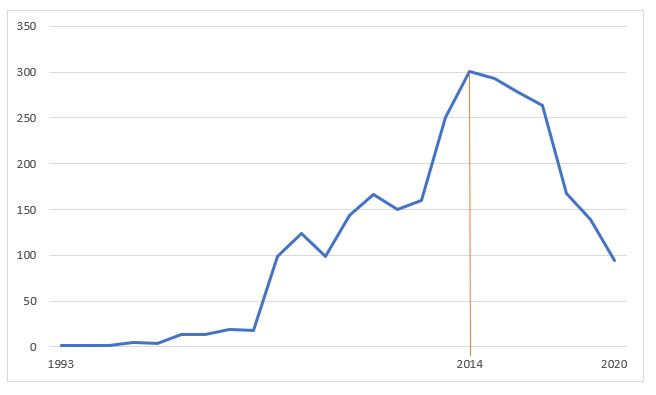
\includegraphics[width=0.7\textwidth]{1.JPG}
    \caption{Caption}
    \label{fig:my_label}
\end{figure}

Otro de los conceptos claves dentro del tema de la mantención industrial, esta la confiabilidad, la cual se refiere a la probabilidad de que un sistema pueda funcionar correctamente fuera de falla por un tiempo específico. Y al igual que la gestión de activos, podemos encontrar un gran numero de investigaciones relacionadas con este tema en particular. Se encuentran cerca de 1.525 investigaciones, entre los años 1996 y 2020. Teniendo el año 2016, el mayor numero de publicaciones con 211.

\begin{figure}[!h]
    \centering
    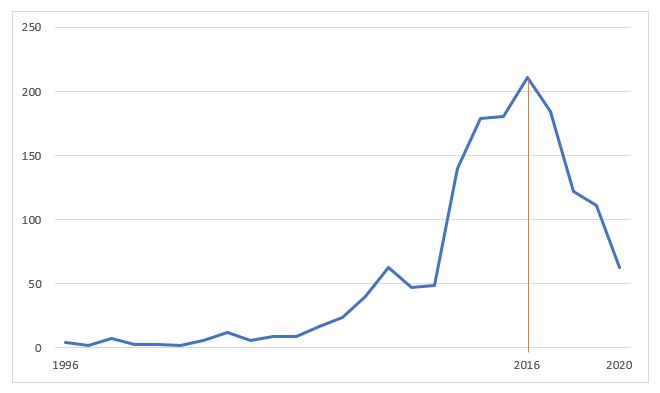
\includegraphics[width=0.7\textwidth]{2.JPG}
    \caption{Caption}
    \label{fig:my_label}
\end{figure}

\hypertarget{marco-conceptual-descripcion-detallada}{%
\section{Marco conceptual}
\label{marco-conceptual-descripcion-detallada}}

\subsection{Disponibilidad}


La disponibilidad es una función que permite estimar en forma global el porcentaje de tiempo total en que se puede esperar que un equipo esté disponible para cumplir la función para la cual fue destinado. A través del estudio de los factores que influyen sobre la disponibilidad, el TPPF y el TPPR, es posible para la gerencia evaluar distintas alternativas de acción para lograr los aumentos necesarios de disponibilidad.\cite{amendola2003indicadores}

\subsection{Confiabilidad}


Es la probabilidad de que un componente o sistema pueda cumplir su función en las condiciones operativas especificadas durante un intervalo de tiempo dado. Esta es la definición general de confiabilidad. Aplica a los componentes o sistemas orientados a una misión y se designa por la letra R. Esta definición no tiene sentido para los componentes o sistemas reparables puesto que éstos toleran las fallas; para estos sistemas se utiliza la disponibilidad.
La probabilidad es la medida clásica para valorar la confiabilidad. Sin embargo, existen muchas otras medidas utilizadas extensamente, por lo cual, “confiabilidad” es un término genérico que describe todas estas medidas sin que necesariamente estén relacionadas con la probabilidad.\cite{rios2014iso}

Es la probabilidad de que un equipo cumpla una misión específica bajo condiciones de uso determinadas en un período determinado. El estudio de confiabilidad es el estudio de fallos de un equipo o componente. Si se tiene un equipo sin fallo, se dice que el equipo es ciento por ciento confiable o que tiene una probabilidad de supervivencia igual a uno. Al realizar un análisis de confiabilidad a un equipo o sistema, obtenemos información valiosa acerca de la condición del mismo: probabilidad de fallo, tiempo promedio para fallo, etapa de la vida en que se encuentra el equipo.
La confiabilidad de un sistema y sus componentes es de suma importancia si queremos conocer la confiabilidad de los activos. Los datos suministrados por los indicadores de confiabilidad debe darnos la distribución de fallos para una o más combinaciones de esfuerzos y ambientes. Uno de los factores a considerar para predecir la confiabilidad de componentes es la tasa de fallo, nivel operativo del equipo, número de ciclos conectados – desconectados, número de horas de funcionamiento, naturaleza y distribución del fallo. Otros aspectos a tomar en cuenta en la configuración de los sistemas es el tipio y grado de redundancia, naturaleza y frecuencia de las acciones de mantenimiento, modos de fallos de componentes sobre sistemas.\cite{zapata2011confiabilidad}

En el siguiente grafico se encuentran las investigaciones que relacionan el tema de disponibilidad y confiabilidad en mantenimiento desde los años 2012 al 2020.


\begin{figure}[!h]
    \centering
    \includegraphics[width=0.7\textwidth]{Figuras/fig2b.png}
    \caption{Disponibilidad y Confiabilidad}
    \label{fig:my_label}
\end{figure}


\subsection{Gestión de Activos}


Actividades y prácticas sistemáticas y coordinadas a través de las cuales una organización administra, de manera óptima y sostenible, sus activos y sistema de activos, su desempeño, su riesgo y costos asociados durante sus ciclos de vida con el propósito de alcanzar su plan estratégico organizacional. Actividades coordinadas de una organización para materializar el valor de sus activos.
La aplicación de un sistema de gestión de activos, bajo los requerimientos establecidos en la ISO 55000, asegura que los objetivos, en cuanto al desempeño de sus activos, serán alcanzados consistente y sosteniblemente en el tiempo, ofreciendo los métodos de control.\cite{amendola2003indicadores}

En el siguiente grafico se encuentran las investigaciones que relacionan el tema de gestión de activos desde el 2005 al 2021.

\begin{figure}[!h]
    \centering
    \includegraphics[width=0.7\textwidth]{Figuras/fig1b.png}
    \caption{Gestion de Activos}
    \label{fig:my_label}
\end{figure}

\hypertarget{contribucion-del-trabajo-identificacion-del-aporte-que-se-hace}{%
\section{Contribución del trabajo}
\label{contribucion-del-trabajo-identificacion-del-aporte-que-se-hace}}
El trabajo del Profesor PhD. Orlando Duran es un modelo que integra el costo de las decisiones, actividades y/o acciones vinculadas con la logística de repuestos con las acciones vinculadas a la gestión de activos, es decir, que las decisiones de gestión de repuestos y las decisiones de mantenimiento estén en un solo modelo.
Se busca identificar cuales son las actividades vinculadas al consumo de cierto recurso (para el caso presentado en clases seria bodega, seguros, personal, etc.). En este modelo, todos los recursos son expresados y son vinculados a las actividades que se desarrollan, es decir, un mapeo de actividades de procesos, donde cada una de las actividades que conforman el proceso están vinculadas como consumidores de ciertos recursos.
Junto a lo anterior, también se busca estiman los costos relacionados con los recursos que se gastan en la logística de repuestos y como se apropian a cada uno de los repuestos que se tienen en una bodega. 



\hypertarget{comentario-adicional}{%
\section{Comentario adicional}
\label{comentario-adicional}}
En mi opinión, la mantención de un activo no solo otorga un beneficio económico para una empresa, sino que además tiene un beneficio medioambiental y social, ya que le estamos otorgando una vida o una utilidad mayor, y podemos ver grandes beneficios de esto. Entre ellos esta la utilización por mas tiempo de una maquinaria, por ejemplo, ahorra la compra o fabricación de otra que realice el mismo proceso, y con esa anulación se obtienen grandes beneficios que van de la mano, como son el gasto energético, de materia prima entre otros. Otro ejemplo seria el  beneficio que podríamos ver el ámbito social, ya que al generar todas estas disminuciones de trabajo y de traslado de grandes equipos de un continente a otro, y podemos logar  minimizamos las emisiones relacionadas al transporte y a la fabricación de cada uno de los componentes, como el traslado total del equipo.





%\hypertarget{referencias}{%
%\section*{Referencias}
%\label{referencias}}
%\addcontentsline{toc}{section}{Referencias}
%\hypertarget{refs}{}

\bibliographystyle{elsarticle-num}
\bibliography{Bibliografia.bib}

\end{document}